\subsection{XGBoost}\label{sec:xgb}
One noteworthy classification method is \emph{Gradient Boosting} and its implementation by Tianqi Chen and Tong Hel via the package \emph{XGBoost}.
After sharing it with other participants early in the challenge, they were rewarded with a special jury-award, for providing "a good compromise between performance and simplicity"\cite{HEPml}. While describing XGBoost, we evaluate this method by these criteria.
For our testing, we use the python package of XGBoost version 0.47 available at \url{https://github.com/dmlc/xgboost}, released on 15. Jan. 2016.

\subsubsection{Boosting}
Assuming, we fit a model to solve a problem. A classifier is called a \emph{strong learner} if it performs well and its prediction achieves a high accuracy. Therefore, a \emph{weak learner} is a classifier that performs poorly, but learns from a training set, the prediction is not made by random guessing.
\emph{Boosting} is the idea to combine a set of weak learners into a single strong learner.

Given training data $x$ with true label $y$, we fit a weak learner $f_1(x)$, which predicts the label $\hat{y}$.
\begin{equation}\label{eq:boosting1}
	y = f_1(x) + z \mathrm{\hspace{1em} ,}
\end{equation}
where $z$ is the prediction error $|y-\hat{y}|$.\\
We replace the error with a second classifier in Eq. \eqref{eq:boosting1} such that
\begin{equation}\label{eq:boosting2}
	y = f_1(x) + f_2(x) \mathrm{\hspace{1em},}
\end{equation}
or equivalently
\begin{equation}\label{eq:boosting3}
	f_2(x) = y - f_1(x) \mathrm{\hspace{1em}.}
\end{equation}
Considering we create an ensemble of weak learners, $f_2$ will not correct $f_1$'s prediction perfectly. To approximate a good \emph{fix} we fit $f_2$ not to the training data $x$, but to the error $y - f_1(x)$, the so-called \emph{residual}.\\
In words: Because our solution is not perfect, we expect an error in our prediction. Therefore, we train another model to fit this error and repeat this process a set number of times.

\subsubsection{Classification method}
Boosting can be trained by minimizing an objective function
\begin{equation}\label{eq:boost_objective}
	L = \sum\limits_{j=1} l ( y_j,F(x_j)) \mathrm{\hspace{1em},}
\end{equation}
where \emph{l} is a loss function, $y_j$ the \emph{true} label of $x_j$ and $F$ is an ensemble of weak learners $\{f_1,f_2,\ldots,f_n\}$. If we use \emph{square loss} as loss function $l$ and differentiate this w.r.t. a weak learner $f_1(x_j)$ of the ensemble such that
\begin{equation}\label{eq:boostloss}
	\frac{\partial l}{\partial f_2(x_j)} = y - f_1(x_j) \mathrm{\hspace{1em},}
\end{equation}
we can observe that $- \frac{\partial l}{\partial f_2(x_j)}$ equals the residual $f_2(x) = y - f_1(x)$.
Thus, residuals of a Boosting model can be interpreted as negative \emph{gradients} that allow minimization of the loss function using \emph{gradient descent}. This is called \emph{gradient boosting}. Further, one can show that a gradient boosting algorithm can be constructed for \emph{any} loss function \cite{gradboost}.

The more complex a classification model is, the higher is the chance of overfitting. Considering this, the main difference of XGBoost to other gradient boosting classifiers is the simple idea to penalize complex models in the ensemble. This is achieved by adding a regularization term $\Omega(f)$, which measures the complexity of $f$, to the objective function Eq.\eqref{eq:boost_objective}. Training this classifier minimizes not only the loss function, but also $\Omega(f_t)$.
The actual predictions are made by weighted \emph{decision trees} with a chosen maximum depth, which are initialized with random values.

We visualize a tree in Fig. \ref{fig:tree} using XGBoost's \emph{plot\_tree} method. It is one of 100 trees fitted to the original training data with a maximum depth of 3.
\begin{figure}[h]
\begin{center}
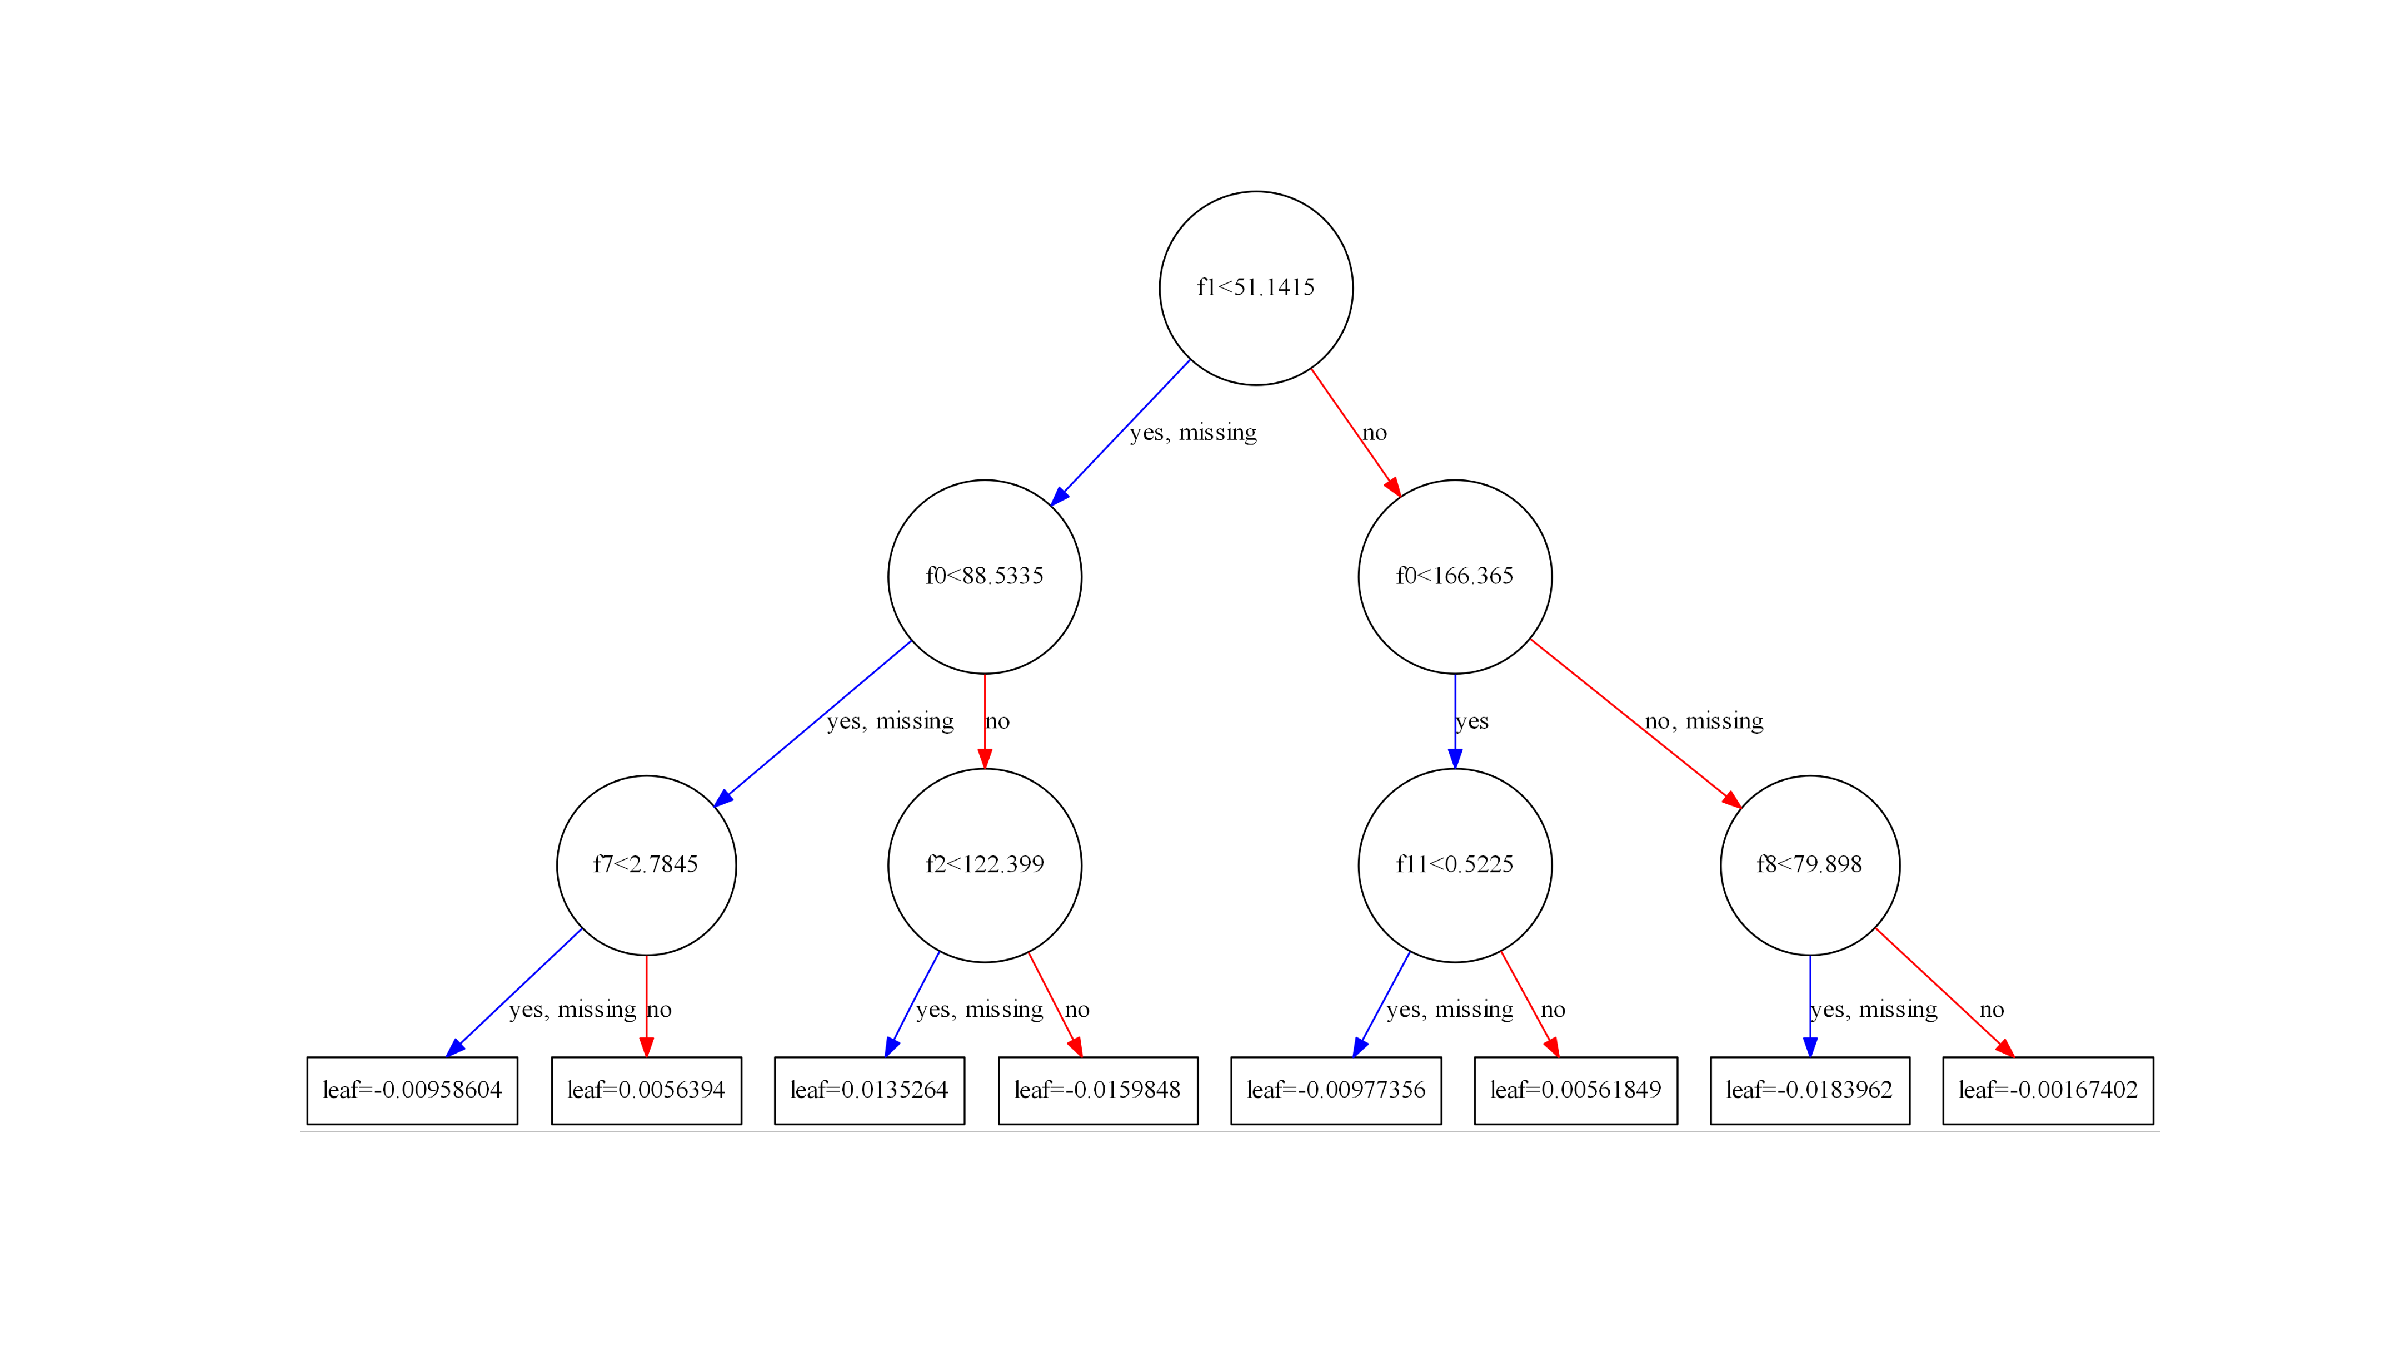
\includegraphics[trim=146 100 118 90, clip, width=\textwidth]{images/tree.pdf}
\caption{A decision tree generated by XGBoost.}
\label{fig:tree}
\end{center}
\end{figure}
\subsubsection{Performance and optimization}
Using default settings, 100 trees and AMS evaluation, XGBoost achieves a public AMS of about 3.32 using the complete, original data set. We get significantly better results by tuning parameters with respect to the public AMS, mainly increasing the number of trees up to 3000 and lowering \emph{eta}. The latter parameter determines the \emph{step size shrinkage} to prevent overfitting. Testing shows that \emph{eta} is inversely related to the tree number, the more trees are used for training, the lower \emph{eta} should be.
Using all parameters, we are still not able to reproduce the exact AMS on the original data stated in \cite{chen14}.
Cutting phi-values, which is suggested by some competitors that use XGBoost \cite{blog}, does not improve the results. Further feature selection fails to resolve into better AMS. Adding artificial features proved beneficial for several submissions using the method.\\
In its recent version, XGBoost provides several alternative objective functions and evaluation metrics. As the package has been developed for the Kaggle challenge, it also contains AMS and AUC as metrics. While the original submission used AUC as model evalutation, we use AUC \emph{and} AMS for training XGBoost with no noticeable disadvantages.

Many software packages implement gradient boosting, as it is an established method in machine learning. While Fig. \ref{fig:xgb-speed} compares speed benchmarks, with all algorithms set up to fit 120 trees with depth 6 and \emph{eta}=0.1, we consider AMS as it is the main goal of the challenge. Since our approaches rely on scikit-learn, we compare the performance of the \emph{GradientBoostingClassifier}(GBC) class to XGBoost , see Fig. \ref{fig:xgb-gbc}.\\
The training GBC consumes over 5000 seconds, while using 100 trees of depth 12. Considering the long training time, we do not perform further training of GBC with more trees. However, it is worth mentioning that the longest training, that was performed on a XGBoost classifier for this thesis, terminated after 1666 seconds, calculating 3000 trees with a depth of 12.
By preprocessing the mathematical model and using decision trees, the training complexity for a tree is reduced to $O(ndK)$ for \emph{n} samples with \emph{d} features, where \emph{K} is the maximum depth of a decision tree\cite{chen14}.

\begin{figure}[h]
\centering
\begin{minipage}[b]{0.48\textwidth}
  \centering
  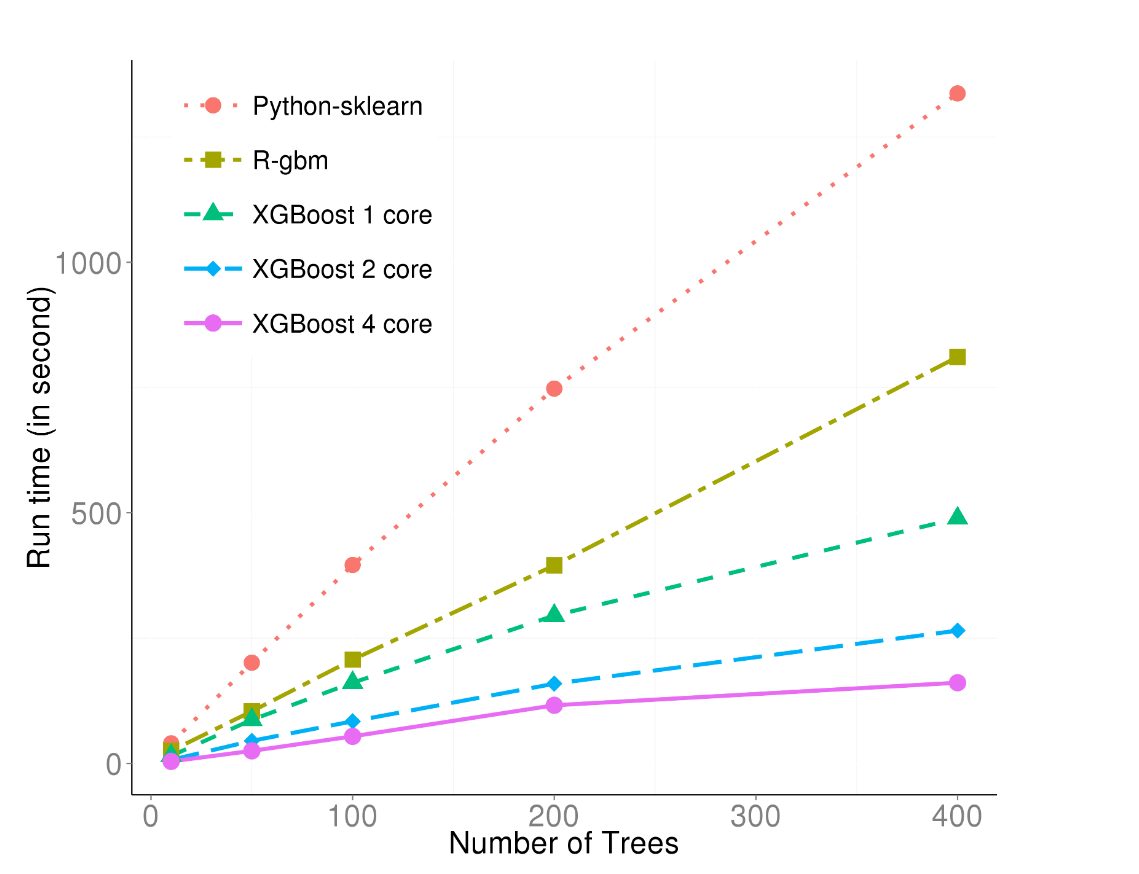
\includegraphics[trim=0 14 60 0,clip,width=\linewidth]{images/xgboost-speed}
  \vspace{-0.1ex}
	\caption{Speed Benchmark on challenge data \cite{chen14}}
	\label{fig:xgb-speed}
\end{minipage}
\quad
\begin{minipage}[b]{0.48\textwidth}
  \centering
  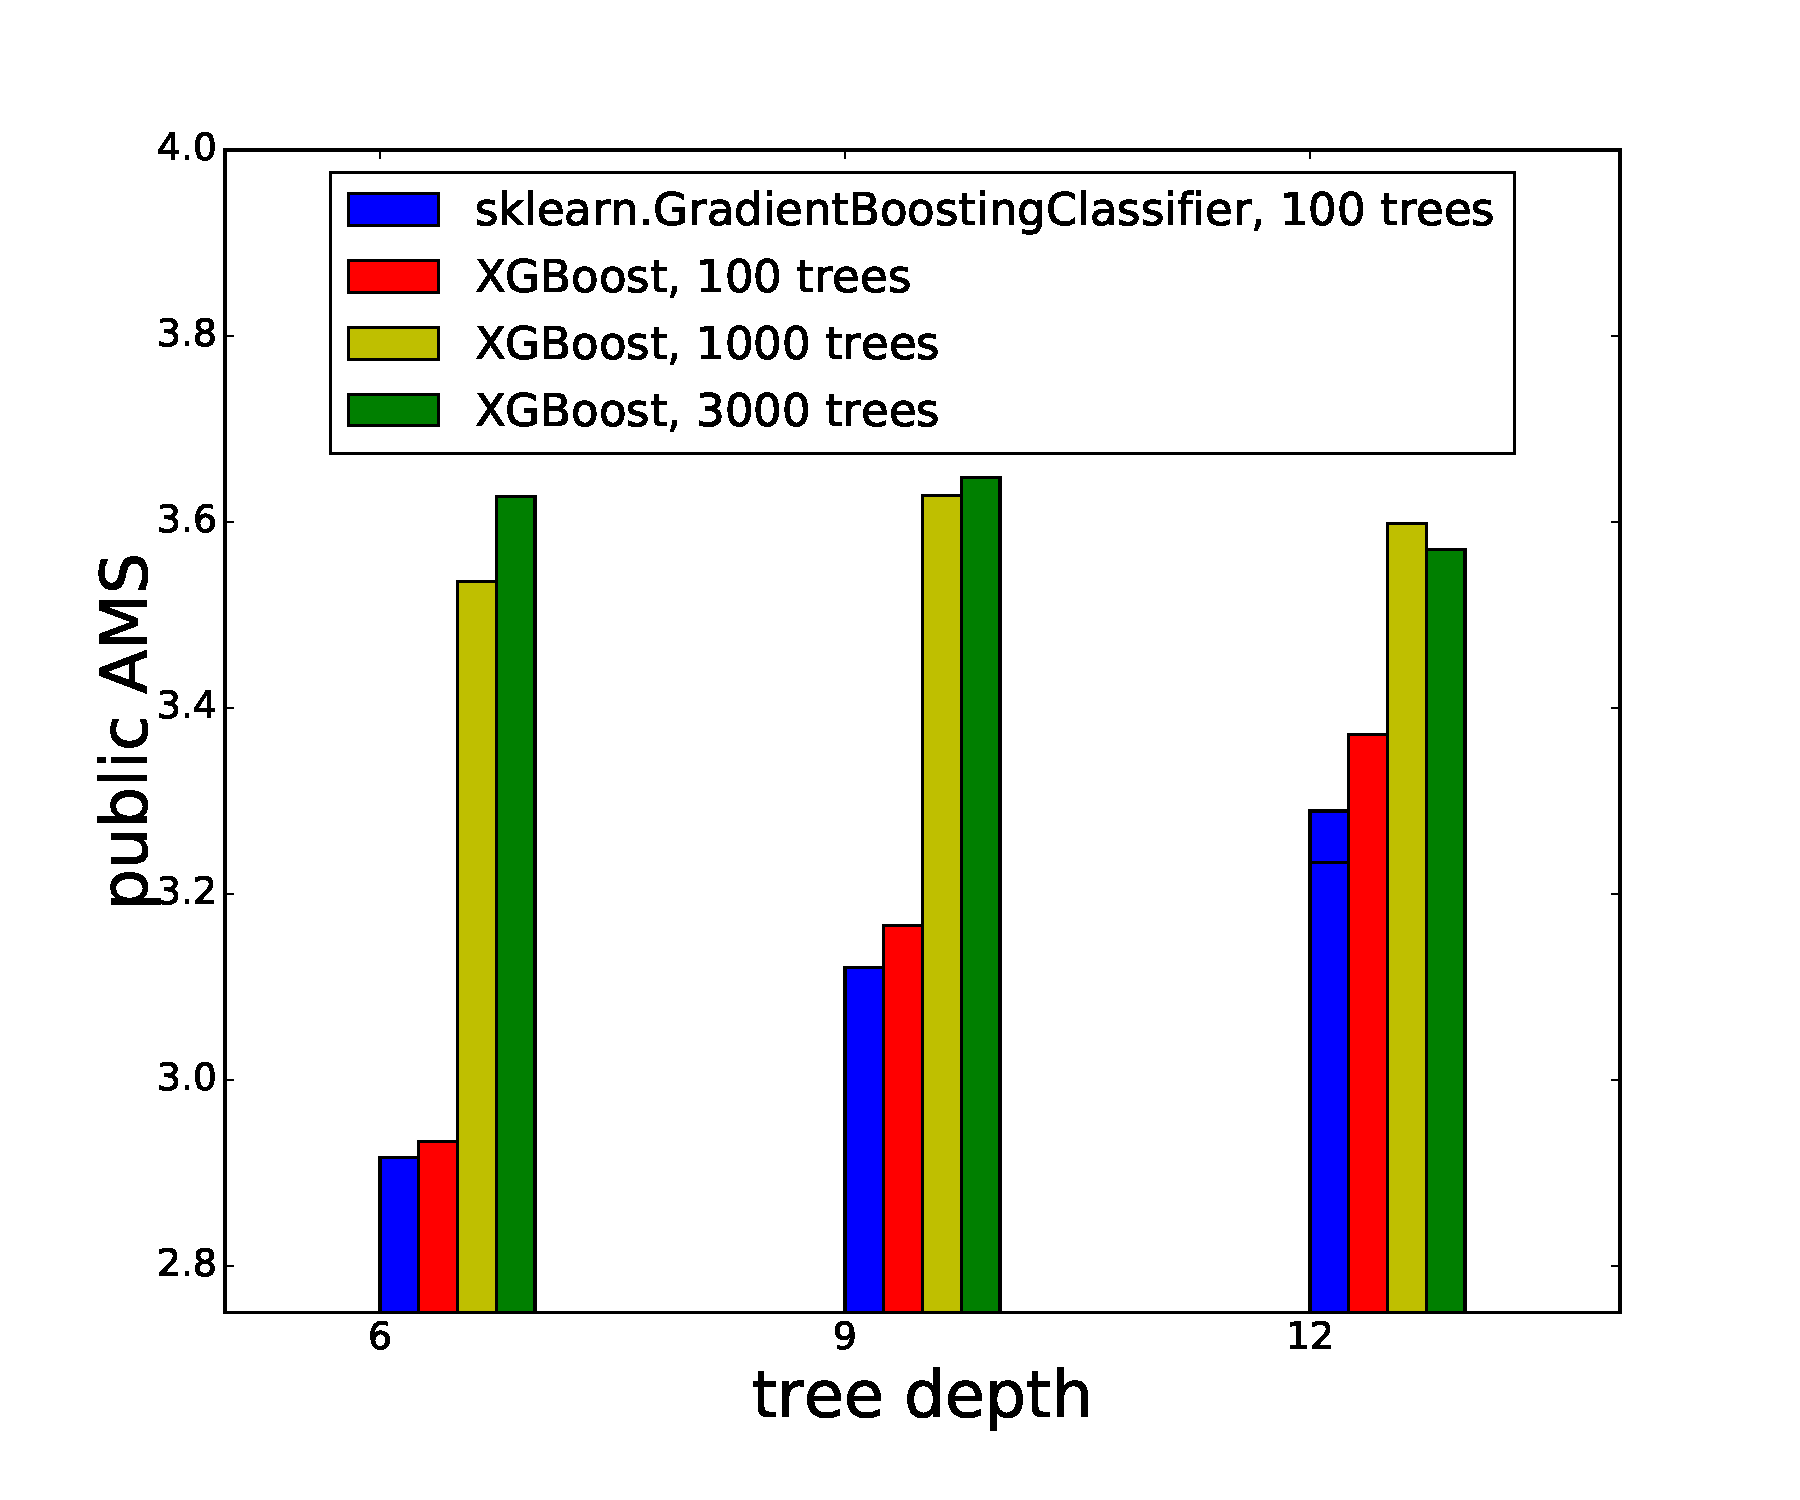
\includegraphics[trim=30 0 40 0,clip,width=\linewidth]{images/xgb-gbc.pdf}
	\caption{AMS-Comparison XGBoost and sklearn.GradientBoostingClassifier}
	\label{fig:xgb-gbc}
\end{minipage}
%\vspace{1ex}
\end{figure}

Regarding the special award, XGBoost seems to fulfil each of its defined aspects. While many other submissions outperform the best benchmark \emph{MultiBoost} easily as well, this package does so remarkably quickly. Training time for a benchmark surpassing result takes under 37 seconds with tuned parameters, using up to 8 CPU threads. This specific run achieved a public AMS of 3.5399.
The developers made the package available early in the challenge and many other participants used it at some point to test custom feature sets or benchmark their own approaches.

It is justified to acknowledge this package, as it could have impact on tools, which are being used in high energy physics\cite{HEPml}.